\subsection{Análise Exploratória dos Dados}
\label{subsec:exploratory_data_analysis}

A visualização gráfica é um método para análise de dados, que permite apresentar características como dispersão e padrões de comportamento, apenas através de dados coletados \cite{wohlin2012experimentation}. A etapa de coleta, consistiu na elaboração de um roteiro que cobrisse todos os possíveis eventos de entrada e saída de um indivíduo em uma instalação, para isso foi elaborado a Tabela \ref{tab:events_description}, que apresenta a numeração de cada evento e sua descrição. Este processo fez-se necessário, pois foi observado maior variação dos dados em eventos que envolviam a interação do indivíduo com a porta da instalação, uma vez que os sensores também captam o movimento da porta.

\renewcommand{\arraystretch}{1.3}
\begin{table}[H]
	\centering
	\caption{Roteiro de Eventos para Etapa de Coleta de Dados}
	\label{tab:events_description}
	\begin{tabular}{|c|c|l|}
		\hline
		\multicolumn{1}{|l|}{\textbf{Evento}} & \multicolumn{1}{l|}{\textbf{Estado Inicial da Porta}} & \multicolumn{1}{c|}{\textbf{Descrição}}                    \\ \hline
		1                                     & Fechada                                               & Abrir a porta, realizar a entrada e fechar a porta.        \\
		2                                     & Fechada                                               & Abrir a porta, realizar a saída e fechar a porta.          \\
		3                                     & Fechada                                               & Abrir a porta, realizar a entrada e manter a porta aberta. \\
		4                                     & Fechada                                               & Abrir a porta, realizar a saída e manter a porta aberta.   \\
		5                                     & Aberta                                                & Realizar a entrada e manter a porta aberta.                \\
		6                                     & Aberta                                                & Realizar a saída e manter a porta aberta.                  \\
		7                                     & Aberta                                                & Realizar a entrada e fechar a porta.                       \\
		8                                     & Aberta                                                & Realizar a saída e fechar a porta.                         \\ \hline
	\end{tabular}
\end{table}

O roteiro de coleta de dados foi executado com seis indivíduos diferentes para que se pudesse observar variações e dispersões em função dos indivíduos e da forma de entrada ou saída de cada um. Para facilitar estas observações, cada evento realizado possui uma gravação de vídeo correspondente, que atua como registro auxiliar durante a etapa de análise dos dados. Desta forma, todo o processo torna-se mais auditável, tendo em vista que o evento armazenado pode ser revisto, ajudando na melhor compreensão de ruídos e \textit{outliers}. A Figura \ref{fig:data_collect} apresenta um conjunto de imagens acerca dos registros de vídeo.

\begin{figure}[ht]
    \center
    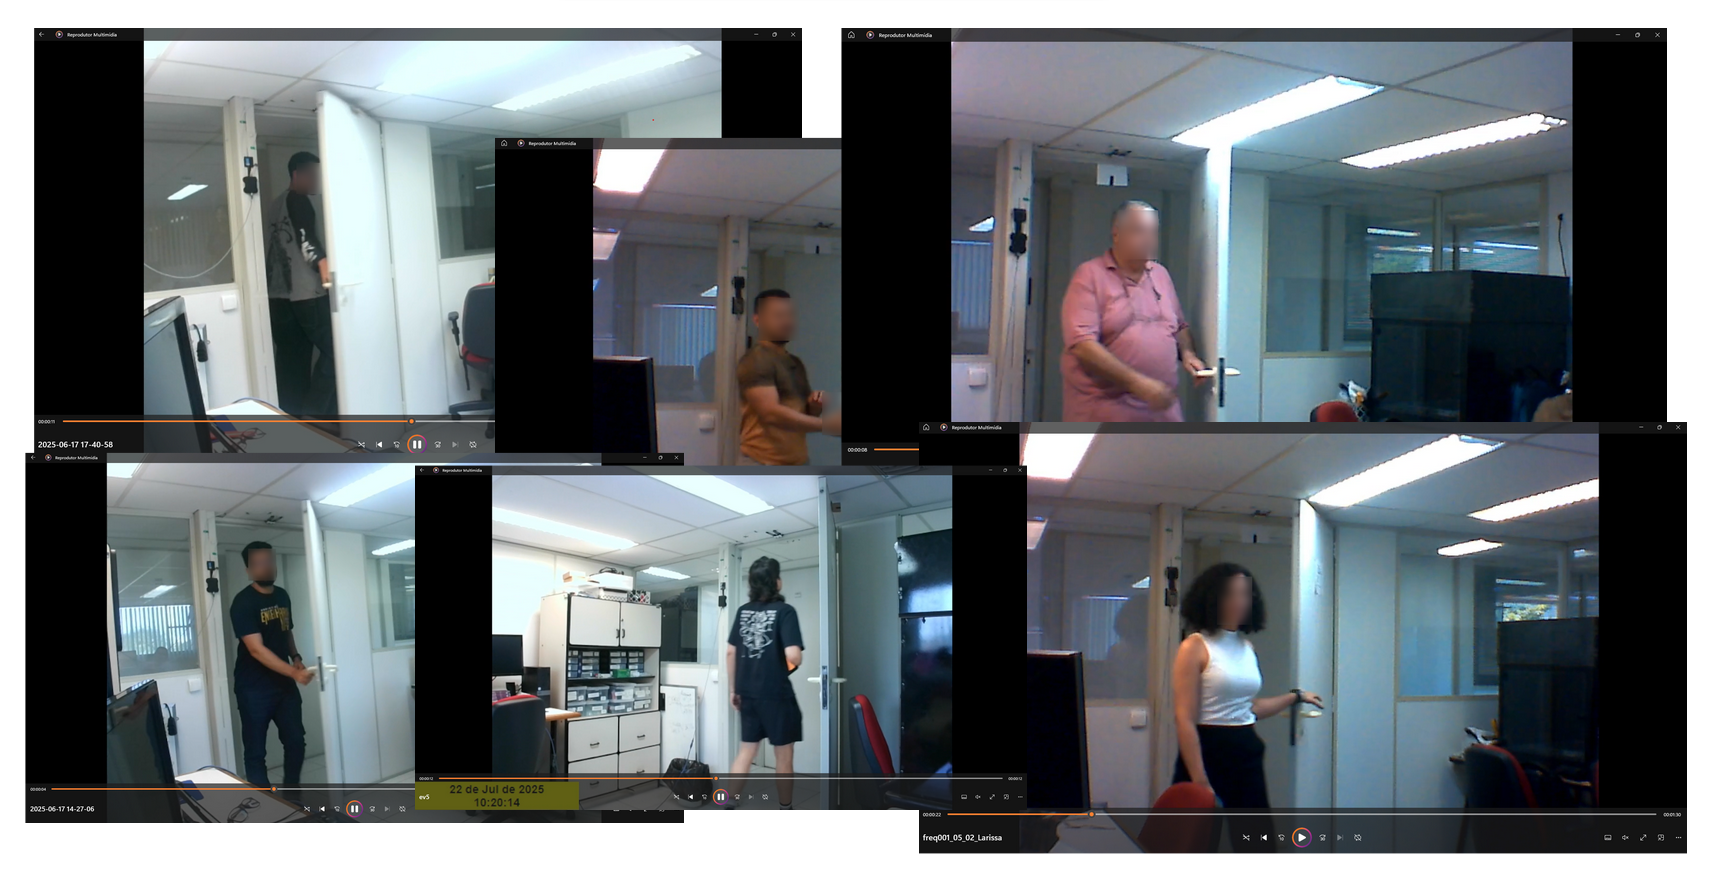
\includegraphics[scale=0.25]{images/data_collect.png}
    \caption{Registros de vídeo realizados durante a coleta de dados}
    \label{fig:data_collect}
\end{figure}

Para a etapa de construção das visualizações gráficas, empregou-se predominantemente a técnica de gráficos bidimensionais de pontos e linhas, conforme ilustrado na Figura \ref{fig:data_visualization}. Essas visualizações representam graficamente os valores de um vetor no eixo y em função de intervalos regulares no eixo x \cite{Komorowski2016}. No contexto da Figura \ref{fig:data_visualization}, o eixo y apresenta os valores de distância medidos pelos sensores ultrassônicos, enquanto o eixo x corresponde ao instante temporal de cada coleta. Além disso, essa abordagem foi adotada pois, em conjunto com os registros de vídeo, permite auditar individualmente cada amostra coletada (representada por um ponto no gráfico), possibilitando a identificação visual de inconsistências, anomalias e medições claramente incompatíveis com o cenário físico observado.


\begin{figure}[H]
    \center
	\fbox{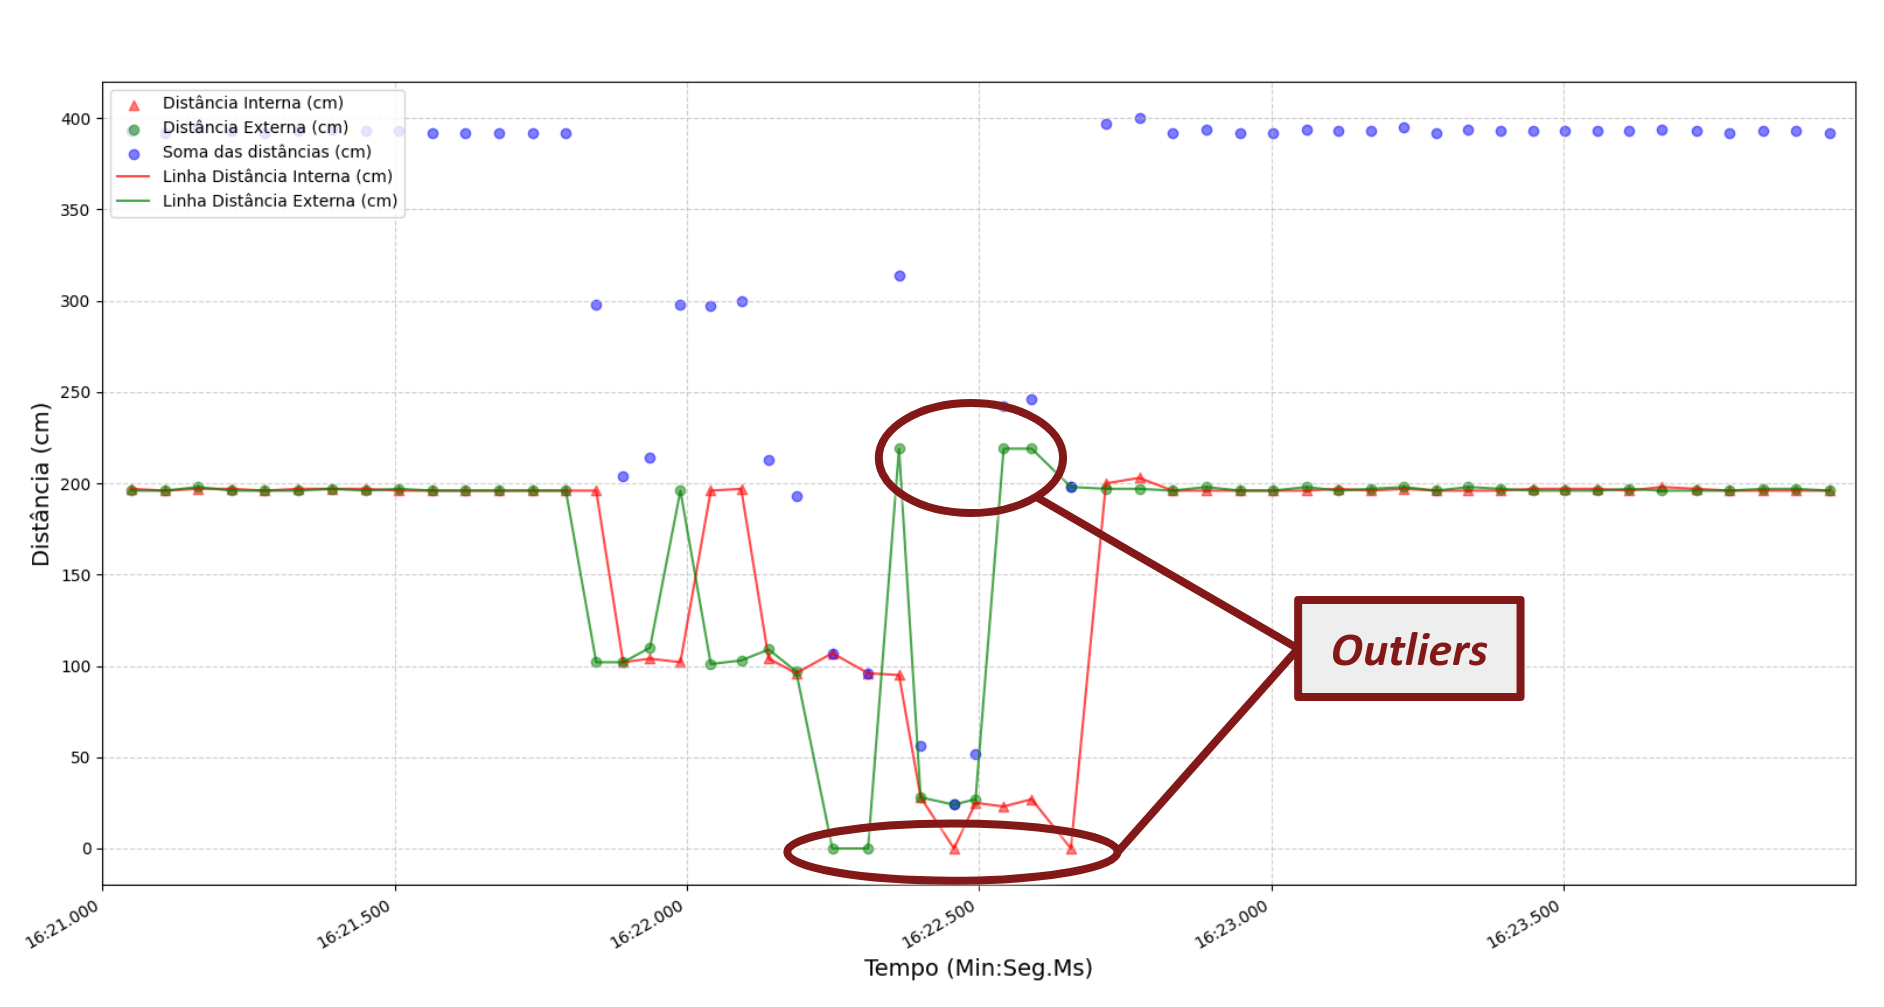
\includegraphics[scale=0.22]{images/datapoints_visualization.png}}
	\caption{Visualização gráfica de um evento de entrada}
	\label{fig:data_visualization}
\end{figure}

A etapa de análise visual dos gráficos apresentou dois padrões de \textit{outliers}, valores superiores a distância total entre os sensores ultrassônicos e o piso, isto é, registros que deveriam ser impossíveis de serem coletados e também valores nulos. O primeiro padrão pode ser justificado devido a interferência entre os dois sensores. Já a ocorrência de valores nulos acontece quando o sensor não consegue captar a onda enviada, isto pode acontecer quando um objeto ou indivíduo impede a propagação da onda, e também caso a onda não seja captada pelo receptor, ocorrência mais comum em objetos com faces irregulares, pois a onda pode ser refletida em direções que não são paralelas ao seu vetor deslocamento inicial, dificultando sua recepção pelo sensor que apenas consegue captar informações em uma região cônica de aproximadamente 45 graus \cite{hcsr04}. 

Além disso, compreende-se que um dos motivos de mal funcionamento do Algoritmo \ref{alg:people_counting} corresponde a ausência de abordagens para lidar com comportamentos irregulares advindos da natureza do sensor utilizado e da estratégia de coleta. A propagação da onda por trajetórias indesejadas é um problema de difícil resolução, tendo em vista que o indivíduo encontra-se em movimento e pode ser interceptado por diversos ângulos. No entanto, existem vários ajustes que podem ser realizados para melhorar a qualidade do evento capturado e consequentemente aprimorar a caracterização pelo sistema. Sendo assim, foram realizados testes para identificar customizações de caráter lógico e físico, que refinassem a coleta de informações, culminando na obtenção de padrões mais constantes e livres de irregularidades. 

\begin{figure}[H]
	\centering

	% --- Primeira linha ---
	\begin{subfigure}[b]{0.48\textwidth}
		\centering
		\fbox{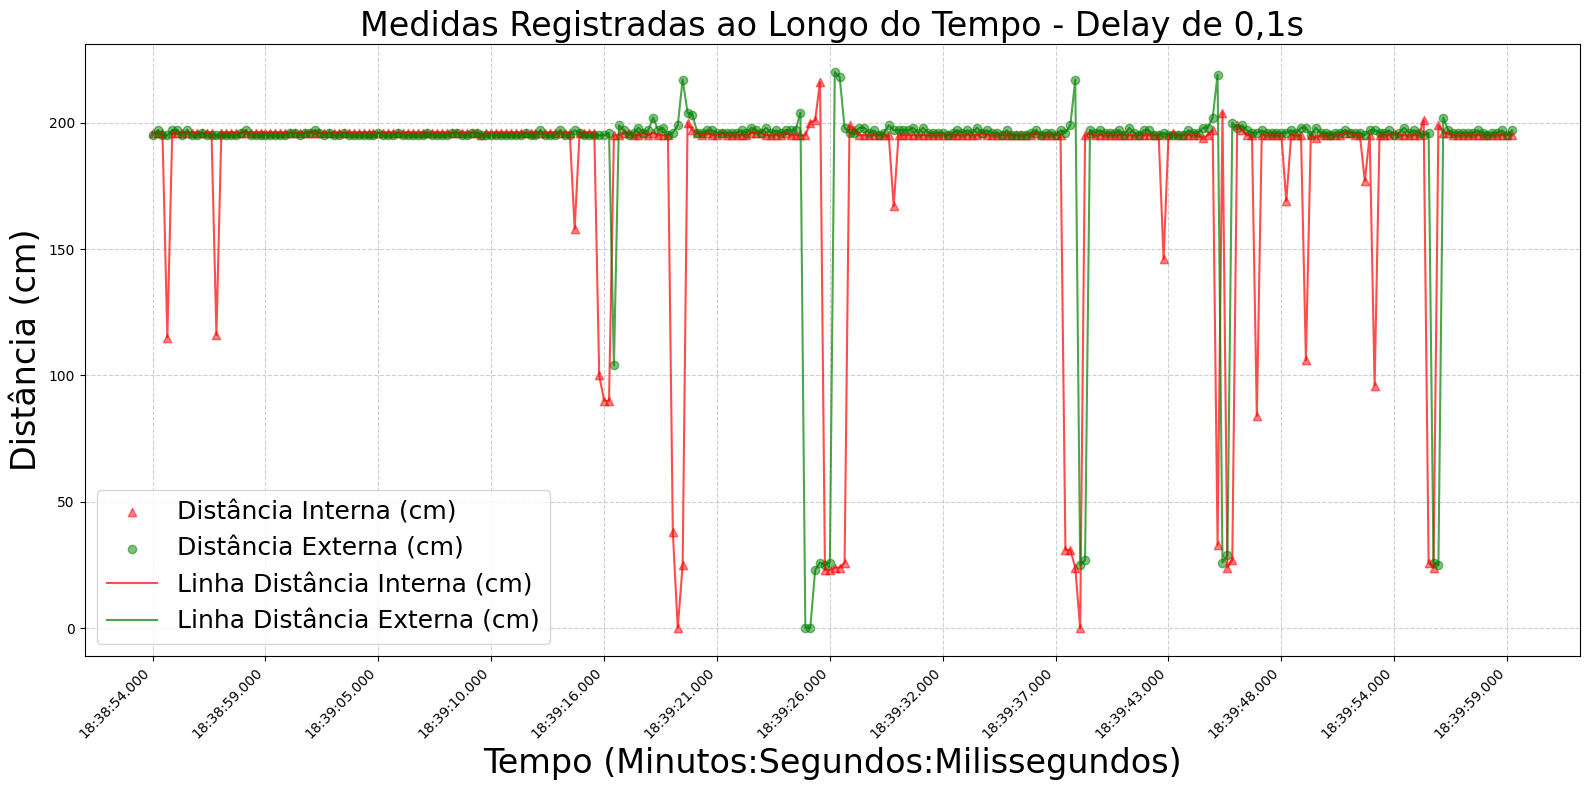
\includegraphics[width=\textwidth]{images/noise_freq_01.png}}
		\caption{Intervalo de 0,1 segundos}
		\label{fig:noise_analysis_01}
	\end{subfigure}
	\hfill
	\begin{subfigure}[b]{0.48\textwidth}
		\centering
		\fbox{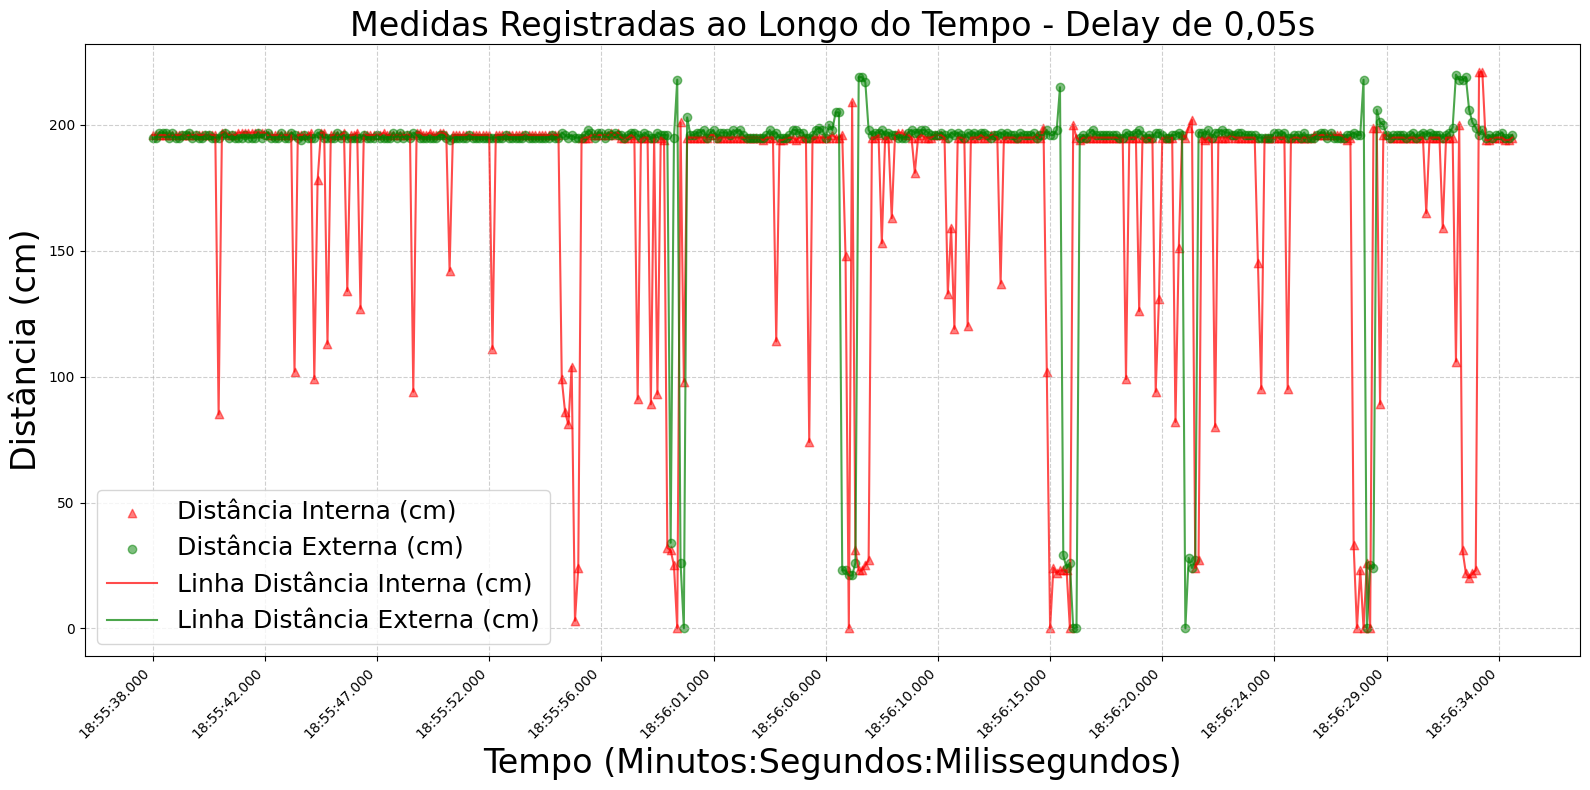
\includegraphics[width=\textwidth]{images/noise_freq_005.png}}
		\caption{Intervalo de 0,05 segundos}
		\label{fig:noise_analysis_005}
	\end{subfigure}

	\vspace{0.4cm}

	% --- Segunda linha ---
	\begin{subfigure}[b]{0.48\textwidth}
		\centering
		\fbox{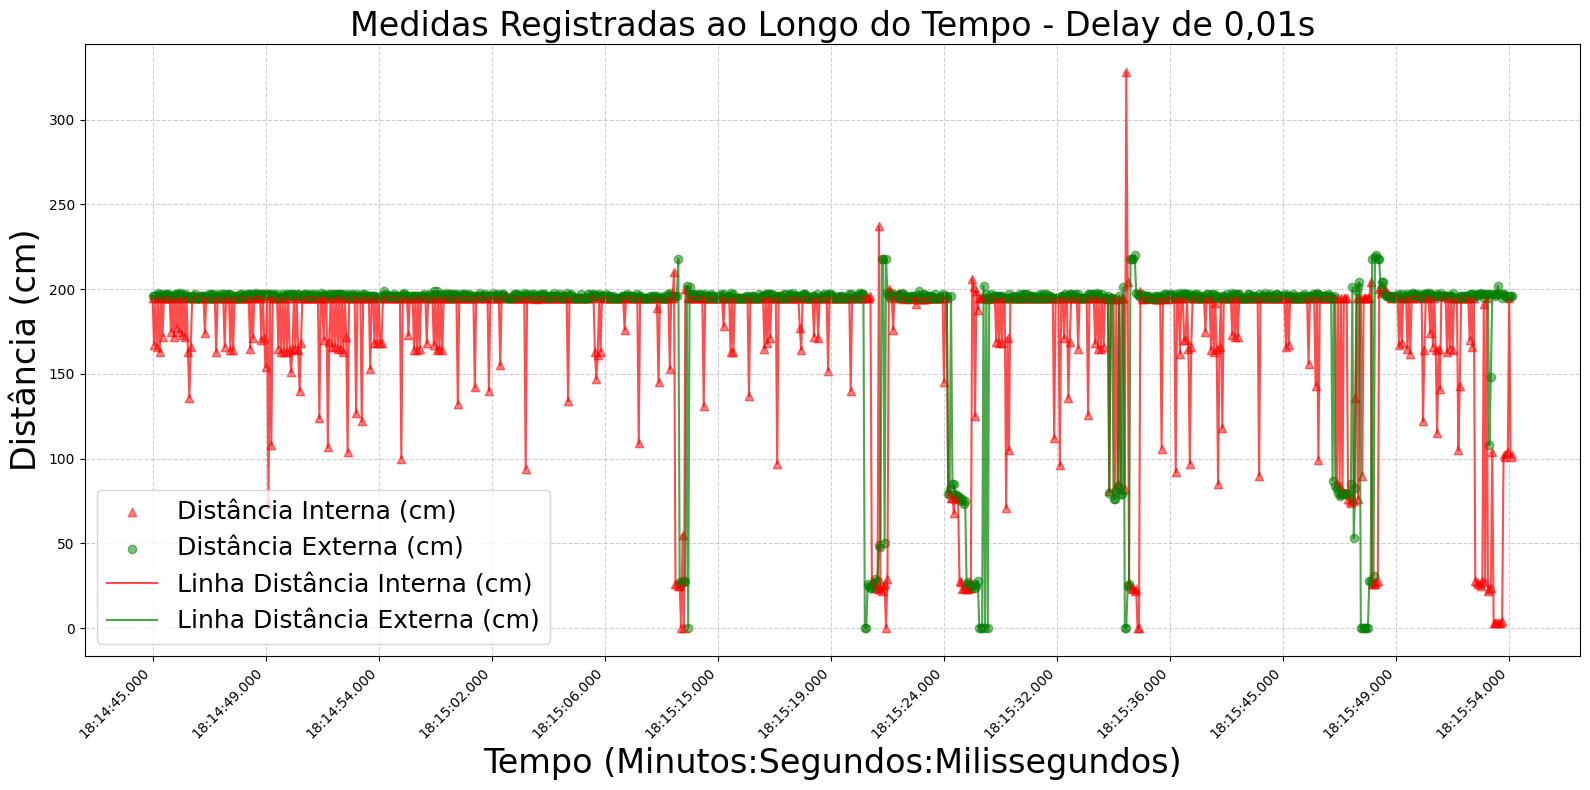
\includegraphics[width=\textwidth]{images/noise_freq_001.png}}
		\caption{Intervalo de 0,01 segundos}
		\label{fig:noise_analysis_001}
	\end{subfigure}

	\caption{Coleta de dados realizadas com intervalos de medição diferentes}
	\label{fig:noise_analysis}
\end{figure}


A fim de determinar o intervalo de coleta que minimiza a interferência entre os sensores, foi realizado uma série de testes com o mesmo dispositivo e nas mesmas condições físicas. Para cada ensaio, variou-se o tempo de espera de cada sensor antes de realizar a sequência de medições. A Figura \ref{fig:noise_analysis} apresenta três gráficos, um para cada intervalo testado, pode-se observar, que ao diminuir o tempo de espera para coleta entre cada sensor, o ruído aumenta de forma quase proporcional. Esse aumento ocorre, pois com um intervalo mais curto a onda emitida por um dos sensores não possui tempo suficiente para se dissipar antes que o outro sensor inicie sua coleta, como as ondas possuem mesma frequência, os sensores não conseguem realizar uma distinção entre elas. Logo, como a distância coletada é calculada através do tempo de deslocamento, caso o sensor receba uma onda que não foi emitida por ele, o valor interpretado será incorreto, pois o \textit{hardware} não sabe lidar com este tipo de situação. 

No entanto, intervalos muito grandes também são um problema, porque a quantidade de dados coletados pode ser insuficiente para categorizar os eventos de interesse. Por fim, o valor adotado foi o de 0,05 segundos, uma vez que apresentou grande diminuição no ruído se comparado ao gráfico de intervalos de 0,01 segundos, bem como obteve caracterização satisfatória de eventos de interesse, diferentemente do gráfico com intervalos de 0,1 segundos.

Outro problema a ser analisado, consiste na dificuldade em identificar eventos de interesse e definir o início e fim destas ocorrências, para posterior análise. Como apresentado nas Figuras \ref{fig:data_visualization} e \ref{fig:noise_analysis} as medidas coletadas não estão livres de interferência entre os sensores, logo a caracterização de eventos de interesse pode ser comprometida. Para lidar com esta problemática, foi acrescentado a parte física do sistema, uma divisória que é anexada a porta da instalação. Sendo assim, sempre que a porta se encontra fechada, a divisória reduz o alcance das ondas propagadas por um dos sensores, retornando sempre uma distância fixa, algo que facilita a busca por padrões de inatividade do sistema. Portanto, ao buscar eventos interesse, basta analisar conjuntos de dados que não correspondem a períodos de inatividade, esta solução facilita a caracterização e poupa processamento, tendo em vista que o sistema não precisa realizar uma análise contínua das medidas coletadas.

Por fim, conclui-se através da análise exploratória dos dados, que o mal funcionamento do módulo de contagem de pessoas corresponde a dois principais fatores: (i) dificuldade em identificar e delimitar conjuntos de dados que compreendam eventos de interesse; (ii) a interferência entre os sensores devido a características inerentes à seu funcionamento. Logo, para que o módulo seja evoluído e seu desempenho aprimorado, deve-se adotar métodos para lidar com estes fatores. 

